\documentclass{article}
\usepackage{tikz}

\begin{document}
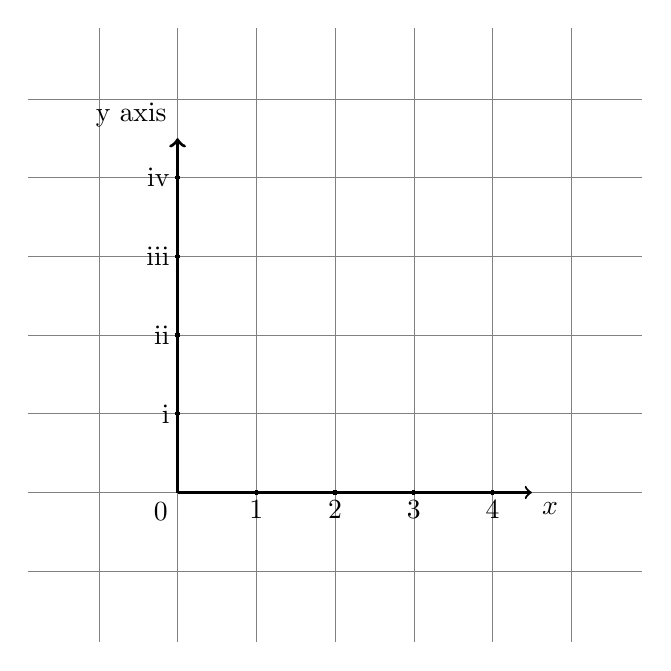
\begin{tikzpicture}
	\draw[step=1cm,gray,very thin] (-1.9,-1.9) grid (5.9,5.9);
	\draw[thick,->] (0, 0) -- (4.5, 0) node[anchor=north west] {$x$};
	% Note that this is for the x-axis and note the sense of the anchor=north west

	\draw[very thick,->] (0,0) -- (0,4.5) node[anchor=south east] {y axis};

	\foreach \x in {1,2,3,4}
		\draw[very thick] (\x cm,-1pt) -- (\x cm,1pt) node[anchor=north] {$\x$};
	\foreach \y in {1,2,3,4}
		\draw[very thick] (-1pt, \y cm) -- (1pt, \y cm) node[anchor=east] {\romannumeral \y};
  \draw (0,0) node[anchor=north east] {$0$};

\end{tikzpicture}
\end{document}
